
%% bare_conf.tex
%% V1.4a
%% 2014/09/17
%% by Michael Shell
%% See:
%% http://www.michaelshell.org/
%% for current contact information.
%%
%% This is a skeleton file demonstrating the use of IEEEtran.cls
%% (requires IEEEtran.cls version 1.8a or later) with an IEEE
%% conference paper.
%%
%% Support sites:
%% http://www.michaelshell.org/tex/ieeetran/
%% http://www.ctan.org/tex-archive/macros/latex/contrib/IEEEtran/
%% and
%% http://www.ieee.org/

%%*************************************************************************
%% Legal Notice:
%% This code is offered as-is without any warranty either expressed or
%% implied; without even the implied warranty of MERCHANTABILITY or
%% FITNESS FOR A PARTICULAR PURPOSE! 
%% User assumes all risk.
%% In no event shall IEEE or any contributor to this code be liable for
%% any damages or losses, including, but not limited to, incidental,
%% consequential, or any other damages, resulting from the use or misuse
%% of any information contained here.
%%
%% All comments are the opinions of their respective authors and are not
%% necessarily endorsed by the IEEE.
%%
%% This work is distributed under the LaTeX Project Public License (LPPL)
%% ( http://www.latex-project.org/ ) version 1.3, and may be freely used,
%% distributed and modified. A copy of the LPPL, version 1.3, is included
%% in the base LaTeX documentation of all distributions of LaTeX released
%% 2003/12/01 or later.
%% Retain all contribution notices and credits.
%% ** Modified files should be clearly indicated as such, including  **
%% ** renaming them and changing author support contact information. **
%%
%% File list of work: IEEEtran.cls, IEEEtran_HOWTO.pdf, bare_adv.tex,
%%                    bare_conf.tex, bare_jrnl.tex, bare_conf_compsoc.tex,
%%                    bare_jrnl_compsoc.tex, bare_jrnl_transmag.tex
%%*************************************************************************


% *** Authors should verify (and, if needed, correct) their LaTeX system  ***
% *** with the testflow diagnostic prior to trusting their LaTeX platform ***
% *** with production work. IEEE's font choices and paper sizes can       ***
% *** trigger bugs that do not appear when using other class files.       ***                          ***
% The testflow support page is at:
% http://www.michaelshell.org/tex/testflow/



\documentclass[conference]{IEEEtran}


\usepackage[final]{pdfpages} 
%
\ifCLASSINFOpdf
  % \usepackage[pdftex]{graphicx}
  % declare the path(s) where your graphic files are
  % \graphicspath{{../pdf/}{../jpeg/}}
  % and their extensions so you won't have to specify these with
  % every instance of \includegraphics
  % \DeclareGraphicsExtensions{.pdf,.jpeg,.png}
\else
  % or other class option (dvipsone, dvipdf, if not using dvips). graphicx
  % will default to the driver specified in the system graphics.cfg if no
  % driver is specified.
  % \usepackage[dvips]{graphicx}
  % declare the path(s) where your graphic files are
  % \graphicspath{{../eps/}}
  % and their extensions so you won't have to specify these with
  % every instance of \includegraphics
  % \DeclareGraphicsExtensions{.eps}
\fi
% graphicx was written by David Carlisle and Sebastian Rahtz. It is
% required if you want graphics, photos, etc. graphicx.sty is already
% installed on most LaTeX systems. The latest version and documentation
% can be obtained at: 
% http://www.ctan.org/tex-archive/macros/latex/required/graphics/
% Another good source of documentation is "Using Imported Graphics in
% LaTeX2e" by Keith Reckdahl which can be found at:
% http://www.ctan.org/tex-archive/info/epslatex/
%
% latex, and pdflatex in dvi mode, support graphics in encapsulated
% postscript (.eps) format. pdflatex in pdf mode supports graphics
% in .pdf, .jpeg, .png and .mps (metapost) formats. Users should ensure
% that all non-photo figures use a vector format (.eps, .pdf, .mps) and
% not a bitmapped formats (.jpeg, .png). IEEE frowns on bitmapped formats
% which can result in "jaggedy"/blurry rendering of lines and letters as
% well as large increases in file sizes.
%
% You can find documentation about the pdfTeX application at:
% http://www.tug.org/applications/pdftex





% *** MATH PACKAGES ***
%
%\usepackage[cmex10]{amsmath}
% A popular package from the American Mathematical Society that provides
% many useful and powerful commands for dealing with mathematics. If using
% it, be sure to load this package with the cmex10 option to ensure that
% only type 1 fonts will utilized at all point sizes. Without this option,
% it is possible that some math symbols, particularly those within
% footnotes, will be rendered in bitmap form which will result in a
% document that can not be IEEE Xplore compliant!
%
% Also, note that the amsmath package sets \interdisplaylinepenalty to 10000
% thus preventing page breaks from occurring within multiline equations. Use:
%\interdisplaylinepenalty=2500
% after loading amsmath to restore such page breaks as IEEEtran.cls normally
% does. amsmath.sty is already installed on most LaTeX systems. The latest
% version and documentation can be obtained at:
% http://www.ctan.org/tex-archive/macros/latex/required/amslatex/math/





% *** SPECIALIZED LIST PACKAGES ***
%
%\usepackage{algorithmic}
% algorithmic.sty was written by Peter Williams and Rogerio Brito.
% This package provides an algorithmic environment fo describing algorithms.
% You can use the algorithmic environment in-text or within a figure
% environment to provide for a floating algorithm. Do NOT use the algorithm
% floating environment provided by algorithm.sty (by the same authors) or
% algorithm2e.sty (by Christophe Fiorio) as IEEE does not use dedicated
% algorithm float types and packages that provide these will not provide
% correct IEEE style captions. The latest version and documentation of
% algorithmic.sty can be obtained at:
% http://www.ctan.org/tex-archive/macros/latex/contrib/algorithms/
% There is also a support site at:
% http://algorithms.berlios.de/index.html
% Also of interest may be the (relatively newer and more customizable)
% algorithmicx.sty package by Szasz Janos:
% http://www.ctan.org/tex-archive/macros/latex/contrib/algorithmicx/




% *** ALIGNMENT PACKAGES ***
%
%\usepackage{array}
% Frank Mittelbach's and David Carlisle's array.sty patches and improves
% the standard LaTeX2e array and tabular environments to provide better
% appearance and additional user controls. As the default LaTeX2e table
% generation code is lacking to the point of almost being broken with
% respect to the quality of the end results, all users are strongly
% advised to use an enhanced (at the very least that provided by array.sty)
% set of table tools. array.sty is already installed on most systems. The
% latest version and documentation can be obtained at:
% http://www.ctan.org/tex-archive/macros/latex/required/tools/


% IEEEtran contains the IEEEeqnarray family of commands that can be used to
% generate multiline equations as well as matrices, tables, etc., of high
% quality.




% *** SUBFIGURE PACKAGES ***
%\ifCLASSOPTIONcompsoc
%  \usepackage[caption=false,font=normalsize,labelfont=sf,textfont=sf]{subfig}
%\else
%  \usepackage[caption=false,font=footnotesize]{subfig}
%\fi
% subfig.sty, written by Steven Douglas Cochran, is the modern replacement
% for subfigure.sty, the latter of which is no longer maintained and is
% incompatible with some LaTeX packages including fixltx2e. However,
% subfig.sty requires and automatically loads Axel Sommerfeldt's caption.sty
% which will override IEEEtran.cls' handling of captions and this will result
% in non-IEEE style figure/table captions. To prevent this problem, be sure
% and invoke subfig.sty's "caption=false" package option (available since
% subfig.sty version 1.3, 2005/06/28) as this is will preserve IEEEtran.cls
% handling of captions.
% Note that the Computer Society format requires a larger sans serif font
% than the serif footnote size font used in traditional IEEE formatting
% and thus the need to invoke different subfig.sty package options depending
% on whether compsoc mode has been enabled.
%
% The latest version and documentation of subfig.sty can be obtained at:
% http://www.ctan.org/tex-archive/macros/latex/contrib/subfig/




% *** FLOAT PACKAGES ***
%
%\usepackage{fixltx2e}
% fixltx2e, the successor to the earlier fix2col.sty, was written by
% Frank Mittelbach and David Carlisle. This package corrects a few problems
% in the LaTeX2e kernel, the most notable of which is that in current
% LaTeX2e releases, the ordering of single and double column floats is not
% guaranteed to be preserved. Thus, an unpatched LaTeX2e can allow a
% single column figure to be placed prior to an earlier double column
% figure. The latest version and documentation can be found at:
% http://www.ctan.org/tex-archive/macros/latex/base/


%\usepackage{stfloats}
% stfloats.sty was written by Sigitas Tolusis. This package gives LaTeX2e
% the ability to do double column floats at the bottom of the page as well
% as the top. (e.g., "\begin{figure*}[!b]" is not normally possible in
% LaTeX2e). It also provides a command:
%\fnbelowfloat
% to enable the placement of footnotes below bottom floats (the standard
% LaTeX2e kernel puts them above bottom floats). This is an invasive package
% which rewrites many portions of the LaTeX2e float routines. It may not work
% with other packages that modify the LaTeX2e float routines. The latest
% version and documentation can be obtained at:
% http://www.ctan.org/tex-archive/macros/latex/contrib/sttools/
% Do not use the stfloats baselinefloat ability as IEEE does not allow
% \baselineskip to stretch. Authors submitting work to the IEEE should note
% that IEEE rarely uses double column equations and that authors should try
% to avoid such use. Do not be tempted to use the cuted.sty or midfloat.sty
% packages (also by Sigitas Tolusis) as IEEE does not format its papers in
% such ways.
% Do not attempt to use stfloats with fixltx2e as they are incompatible.
% Instead, use Morten Hogholm'a dblfloatfix which combines the features
% of both fixltx2e and stfloats:
%
% \usepackage{dblfloatfix}
% The latest version can be found at:
% http://www.ctan.org/tex-archive/macros/latex/contrib/dblfloatfix/




% *** PDF, URL AND HYPERLINK PACKAGES ***
%
%\usepackage{url}
% url.sty was written by Donald Arseneau. It provides better support for
% handling and breaking URLs. url.sty is already installed on most LaTeX
% systems. The latest version and documentation can be obtained at:
% http://www.ctan.org/tex-archive/macros/latex/contrib/url/
% Basically, \url{my_url_here}.




% *** Do not adjust lengths that control margins, column widths, etc. ***
% *** Do not use packages that alter fonts (such as pslatex).         ***
% There should be no need to do such things with IEEEtran.cls V1.6 and later.
% (Unless specifically asked to do so by the journal or conference you plan
% to submit to, of course. )


% correct bad hyphenation here
\hyphenation{op-tical net-works semi-conduc-tor}


\begin{document}
%
% paper title
% Titles are generally capitalized except for words such as a, an, and, as,
% at, but, by, for, in, nor, of, on, or, the, to and up, which are usually
% not capitalized unless they are the first or last word of the title.
% Linebreaks \\ can be used within to get better formatting as desired.
% Do not put math or special symbols in the title.
\title{Towards a unified workflow for multi contact motion on legged robots: Challenges in planning, optimization and control.}

%~ \title{\vspace{-4ex}Towards a unified workflow for multi contact motion on legged robots: Challenges in planning, optimization and control.}
%~ \author{Organizers:
	%~ Name 1,
	%~ Name 2,
	%~ Name 3\\
	%~ Directorate Liaison: Name of Liaison}
%~ \date{Dates in 20??, at SAMSI}
\maketitle

%~ \noindent
%~ A proposal for a SAMSI workshop should contain the following items.

\section{\textbf{Title} of proposed workshop}
Towards an unified workflow for multi contact motion or legged robots: Challenges in planning, optimization and control.

\section{Duration of the workshop}
Full-Day Workshop.

\section{Organizers}
\subsection*{Steve Tonneau: primary contact person}
\textbf{affiliation}: Post doctorate researcher at LAAS-CNRS.

\textbf{address}: 7 avenue du Colonel Roche, 31400 Toulouse

\textbf{phone}: (+33) 5-61-33-68-90

\textbf{email}: stonneau@laas.fr
\textbf{url}: http://stevetonneau.fr
\subsection*{Timothy Bretl}
\textbf{affiliation}: Associate Professor of Aerospace Engineering,

 University of Illinois

\textbf{address}: 148 Coordinated Science Laboratory, MC-228,

 1308 West Main Street, Urbana, IL, 61801-2307, USA 

\textbf{phone}: 217-244-3126 

\textbf{email}: tbretl@illinois.edu 
\textbf{url}: http://bretl.csl.illinois.edu

\subsection*{Nicolas Mansard}
\textbf{affiliation}: Permanent researcher at LAAS-CNRS.

\textbf{address}: 7 avenue du Colonel Roche, 31400 Toulouse

\textbf{phone}: (+33) 5-61-33-68-90

\textbf{email}: nicolas.mansard@laas.fr

\textbf{url}: http://homepages.laas.fr/nmansard

\subsection*{Igor Mordatch}
\textbf{affiliation}: Post-doctoratl fellow 

University of California, Berkeley.

\textbf{address}: 750 Sutardja Dai Hall, Berkeley, CA 98195

\textbf{phone}: (+1) 510 459 3152

\textbf{email}: mordatch@berkeley.edu

\textbf{url}: http://www.eecs.berkeley.edu/~igor.mordatch/


\section{Website url}
http://homepages.laas.fr/nmansard/entracte/

index.php?n=Publication.WorkshopIcra2015

\section{\textbf{Abstract}}
Early contributions on multi contact locomotion for legged robots have underlined the complexity of planning and executing motions in cluttered environments. In both the robotics and computer-graphics community, a large variety of approaches have been recently proposed to tackle the problem, thus often targeting one specific aspect: the planning of a feasible path for the robot, the optimization of its trajectory, or the feedback control of the robot during
the execution of a dynamic motion. Integrating these different aspects is not only an engineering issue. It raises scientific questions in terms of robustness of the algorithms and performance requirements. The objective of this workshop is to gather people working in these fields and propose a debate on the combination of these various aspects into a functional workflow for robot motions in cluttered environments.
Renowned speakers from the robotics and computer graphics field will present their work, and recommend the reading of selected papers prior the conference.  This will provide the audience with the ability to prepare their venue and ask relevant questions that will be analyzed by student groups and discussed during dedicated debate sessions.


\section{Content}
\subsection{Situation of the problem}
Achieving multi-contact locomotion is challenging: Theoretically, the motion or manipulation planning problem is known to be particularly difficult due to the complex topology of the configuration space. In practice, the execution of a planned trajectory on a robot requires the resolution of the problem of moving in contact while maintaining the balance of an underactuated unstable system. 

This problem is recognized by both the robotics and computer-graphics community, and their respective approaches have a lot to share.
It has gained visibility and interest with the advent of humanoid and legged robots, and in particular with the DARPA Robotics Challenge. While impressive advances have been emphasized, the challenge also shown that legged robots are far to be as mature as wheeled robots.

The problem can be roughly divided in three aspects. At the planning level, it is often considered to compute a discrete sequence of statically balanced key contact postures. In a second level, the complete continuous trajectory connecting all the postures is considered. The last level considers the control law that executes the complete movement on the robot despite the uncertainties of the model. These three aspects of the problem are strongly correlated and might be treated separately to reduce the complexity or together to provide a better approximation of a targeted optimality.

\subsection{Objective}
The workshop aims at gathering the key researchers studying all the three aspects of the problem, to provide an exhaustive painting of the state of the art, the current blocking problems and the future promising directions. One originality is that we have brought several key researchers from the computer-graphics community to share their viewpoints with the roboticists.

\subsection{Organization of the day}
The workshop consists in three topic specific presentation sessions, completed by two inter topic debate/poster sessions. These sessions are organized in an original fashion so as to enhance exchange and communication: the talks of each session will be completed with a topic specific
debate session, prepared by students.
A few months before the workshop, each presenter will recommend the reading of one or two papers, available on the workshop website. 
The students will read the paper, collect questions asked online by the public, and prepare a critic presentation of the papers that will start the debate session. Additionally, the audience will be given the opportunity to ask questions in real time using social networks during presentations.

An inter topic poster session aims at connecting two topic specific research issues, namely motion planning / trajectory generation and trajectory generation / robot control, and will result from a call for poster contributions.

We propose the following planning tentative: \\

\textbf{08.30}: Welcoming and introduction

\textbf{08.40}: Motion planning: 3 talks + topic debate

\textbf{10.25}: Coffee break

\textbf{10.40}: Trajectory optimization: 3 talks + topic debate

\textbf{12.25}: Dinner break

\textbf{13.25}: Poster session 1

\textbf{14.25}: Robot feedback control: 3 talks + topic debate

\textbf{16.15}: Poster session 2

\textbf{17.15}: Conclusion and farewell
%~ 
%~ The topics covered are:
%~ \begin{itemize}
%~ \item Motion and contact planning in cluttered environments
%~ \item Generation of contact trajectories through optimization
%~ \item Feedback control for executing multi contact motions on actual robots
%~ \end{itemize}
%~ 
%~ The debate sessions aim at discussing the specific issue of connecting these three topics so as to obtain a fully functional workflow from the planning to the robot.
%~ 
%~ A presentation session covers a specific aspect of multi contact planning for robots and  consists in:
%~ A long review talk (35 min)
%~ 2 specific talks (15 min each)
%~ A topic specific debate session, animated by a group of students
%~ 
%~ The topic specific debate is prepared before the event by the students, according to an agenda:
%~ A few months before the workshop, each presenter will recommend the reading of one or two papers, available on the workshop website. 
%~ The students will read the paper, collect questions asked online by the public, and prepare a critic presentation of the papers that will start the topic specific debate session. 
%~ Additionally, the audience will be given the opportunity to ask questions in real time using social networks.
%~ 
%~ An inter topic poster session aims at connecting two topic specific research issues, namely motion planning / trajectory generation and trajectory generation / robot control. They will have the following form:
%~ A “fast forward” session, where the authors of poster will present a teaser of their poster in two minutes;
%~ The actual poster session, resulting from a call for contributions, will follow on these specific aspects.



\section{List of confirmed speakers}
%~ Because of the time constraints of some of the invited speakers, we ask that the workshop happens on the second day.

All the indicated speakers have confirmed their presence, although not all of them have been able to provide us with a title and / or abstract
of their presentation.\\ \\
\textbf{Speaker}: Russ Tedrake, MIT, USA \\
\textbf{Title}:  Robust feedback stabilization through unscheduled contact.\\
\textbf{Abstract}: The talk will be a synthesis of the work performed in my lab during the last 5 years on the generation of locomotion movements in contact with the environment. In particular, the presentation would cover and connect the following recent results:
\begin{itemize}
\item selection of contact locations formalized as mixed-integer optimization;
\item generation of whole-body movements in contact, in particular simultaneous optimization of kinematics and  central dynamics;
\item planning and control of locomotion from dense perception \\ \\ 
\end{itemize}
%~ 
\textbf{Speaker}: Antonio Bicchi, University of Pisa, Italy\\
\textbf{Title}: TBD \\
\textbf{Abstract}: TBD \\ \\
%~ 
\textbf{Speaker}: Shunichi Nozawa, The university of Tokyo, Japan \\
\textbf{Title}:  Planning and execution of whole-body environment and object
manipulation with a life-sized humanoid robot \\
\textbf{Abstract}: In this presentation, we introduce planning and execution system for whole-body environment and object manipulation with a life-sized humanoid robot by adaptive selecting of manipulation strategy and robust motion execution through haptic sensing of actual contact states and object's motion. \\ \\
%~ 
\textbf{Speaker}: Siddhartha Srinivasa, Carnegie Mellon University \\ 
\textbf{Title}: Physics-based manipulation under clutter and uncertainty \\
\textbf{Abstract}: My research goal is to bridge the gap between what robots can do now and what they are capable of doing. Towards that goal, I will overview some of our recent work on (1) using physics to increase the repertoire of manipulation actions beyond pick-and-place to nonprehensile and whole-arm manipulation, (2) orchestrating this repertoire to reconfigure clutter, (3) using physics to funnel uncertainty via open-loop robust controllers, and (4) representing uncertainty via state estimators and reducing uncertainty via information-seeking actions. \\ \\
%~ 
\textbf{Speaker}: Adrien Escande, CNRS/AIST, JRL, Tsukuba, Japan \\
\textbf{Title}: Multi-contact motion planning for humanoid robots: from theory to experiments \\ 
\textbf{Abstract}: This talk will give an overview of several important aspects of multi-contact planning and control. First the problem of planning a sequence of postures in contact with the environment will be discussed through an academic example that contains most of the conceptual complexity. An effective algorithm to compute such a sequence will then be presented, able for example to compute a sequence for a humanoid robot to climb a vertical ladder. From planning to execution, we need to solve various numerical problems. We will in a second part highlight the robotics specificities of these problems (variables living on non-Euclidean manifolds, hierarchy of objectives) and discuss some ways to solve them more efficiently/easily than with classical methods. We will then show how the new solvers enable us to formulate richer problems. \\ \\
%~ 
\textbf{Speaker}: Patrick Wensing, MIT, USA \\
\textbf{Title}:  Addressing force optimization through simple models: reflections on applications across humanoid and quadruped robots \\
\textbf{Abstract}:  This talk will focus on the use of force optimization with simple models as an enabling component for dynamic mobility in robots of different morphologies. As our robots move through complex environments, they will increasingly need to consider the limited control authority provided through friction-limited contacts in developing their motion plans.  To handle these challenges for dynamic operating regimes, I will discuss simple models across humanoid and quadruped robots with focus on their unifying characteristics.  With this outlook, I will demonstrate real-time control for robust locomotion across uneven terrain in humanoids, and extreme mobility in the MIT Cheetah.\\ \\
%~ 
\textbf{Speaker}: Quang-Cuong Pham, Nanyang Technological University, Singapore \\
\textbf{Title}:  Revisiting and extending ZMP to multiple non-coplanar contacts \\
\textbf{Abstract}: We argue that the correct viewpoint to understand the ZMP is that of weak contact stability. Based on that viewpoint and the Cone Double Description technique, we could extend ZMP to multi-contact by computing its support area in arbitrary virtual planes. Testing the dynamic equilibrium of a humanoid robot then simply boils down to checking that the ZMP computed in the virtual plane belongs to the corresponding support area. Based on these developments, we implement a whole-body controller and generate dynamically-stable motions where an HRP-4 humanoid locomotes in challenging simulation environments.   \\ \\
%~ 
\textbf{Speaker}: Igor Mordatch, University of California, Berkeley USA \\
\textbf{Title}: From trajectory optimization to model learning for the locomotion of virtual characters and humanoids robots \\
\textbf{Abstract}: This talk will present two contributions emblematic of recent approaches to the issue of planning dynamic trajectories for humanoid robots.
First, I will describe Contact Invariant Optimization (CIO), a fully automatic approach for motion generation, which does not require domain knowledge specific,
and enables simultaneous optimization of contact and behavior. I will elaborate on Ensemble-CIO, an improvement of the CIO that makes it robust to  perturbations on the perception
and control of the actual robot. Secondly, I will describe my most recents contributions that make use of both offline and online model learning algorithms to make real-time motion generation
achievable on real robots.  \\ \\
%~ 
\textbf{Speaker}: Steve Tonneau, LAAS CNRS, France \\
\textbf{Title}: Interactively planning truly feasible contact sequences for legged virtual characters and robots.\\
\textbf{Abstract}: Recent progress in multi contact planning hold the promise of interactively generating feasible plans for legged robots, executed on the fly.
However, existing multi contact planners do not sufficiently take into account the dynamic limitations of the robots for which the planning is performed, nor for the uncertainties of the environment. The sad truth is that in cluttered environments, executing a planned motion is at best extremely hard, at worst simply impossible. Introducing such
robustness into modern contact planners is thus a necessary condition for the design of a complete, unsupervised
motion synthesis framework that will truly provide legged robots with motion autonomy. I will
present the latest results obtained in the domain of robust contact planning, and discuss the most exciting perspectives
in this regard.\\ \\

\section{Plan to solicit participation}
The recent popularity of research in Multi contact planning, illustrated by events such as the Darpa Challenge, goes beyond the field of robotics, with collaborations in the computer graphics community. In the last five years several papers have been the highlight of the highly renowned SIGGRAPH conference, and Karen Liu, author of several of them, is one of our key speakers. This will provide the workshop with a strong visibility in this community.

Similarly, the list of confirmed speakers include some of the most renowned researchers in robotics.
The workshop format is a unique chance for researchers, especially young students, to collaborate and exchange with the speakers.

Because it is multidisciplinary and aims at creating synergies between researchers from motion planning, optimization and control, and character animation for computer graphics, we expect an important attendance.

\section{Plan to encourage interaction among participants}
One originality of the workshop lies in the fact that prior to the conference, a reading list will be given online, allowing people to prepare and submit their questions in advance. This aspect was appreciated by invited speakers such as Russ Tedrake, and we believe that the work produced prior to the conference will encourage on site discussion.

The workshop is also organized in a way that allow speaking time to established researchers, but also young students which will have prepared their interventions and be less intimidated to speak in public.

Furthermore, during the presentations the audience will be given the opportunity to ask questions online using twitter or the conference website. These questions will be in turn asked by the organizers during he dedicated debate sessions.

\section{Equipments}
In addition to standard equipment we
anticipate the need of a number of 20 poster interactive screens
or stands.

\section{Support of an IEEE RAS Technical Committee}
The workshop is supported by the Whole Body Control Technical Commitee, represented by Dr. Luis Sentis.
It is also supported by Prof. Dr. Katja Mombaur, chair of the Technical Comitee on Model-based Optimization.

\section{Attachements}
Attached to this proposal are:
\begin{itemize}
\item The letters of support from the Whole Body Control and Model-based Optimization TC;
\item The history of email exchange with the confirmed speakers, proving that they accepted to talk.
The relevant parts of these long logs are underlined. The two remaining speakers, Steve Tonneau and Igor Mordatch,
are members of the organization.
\end{itemize}

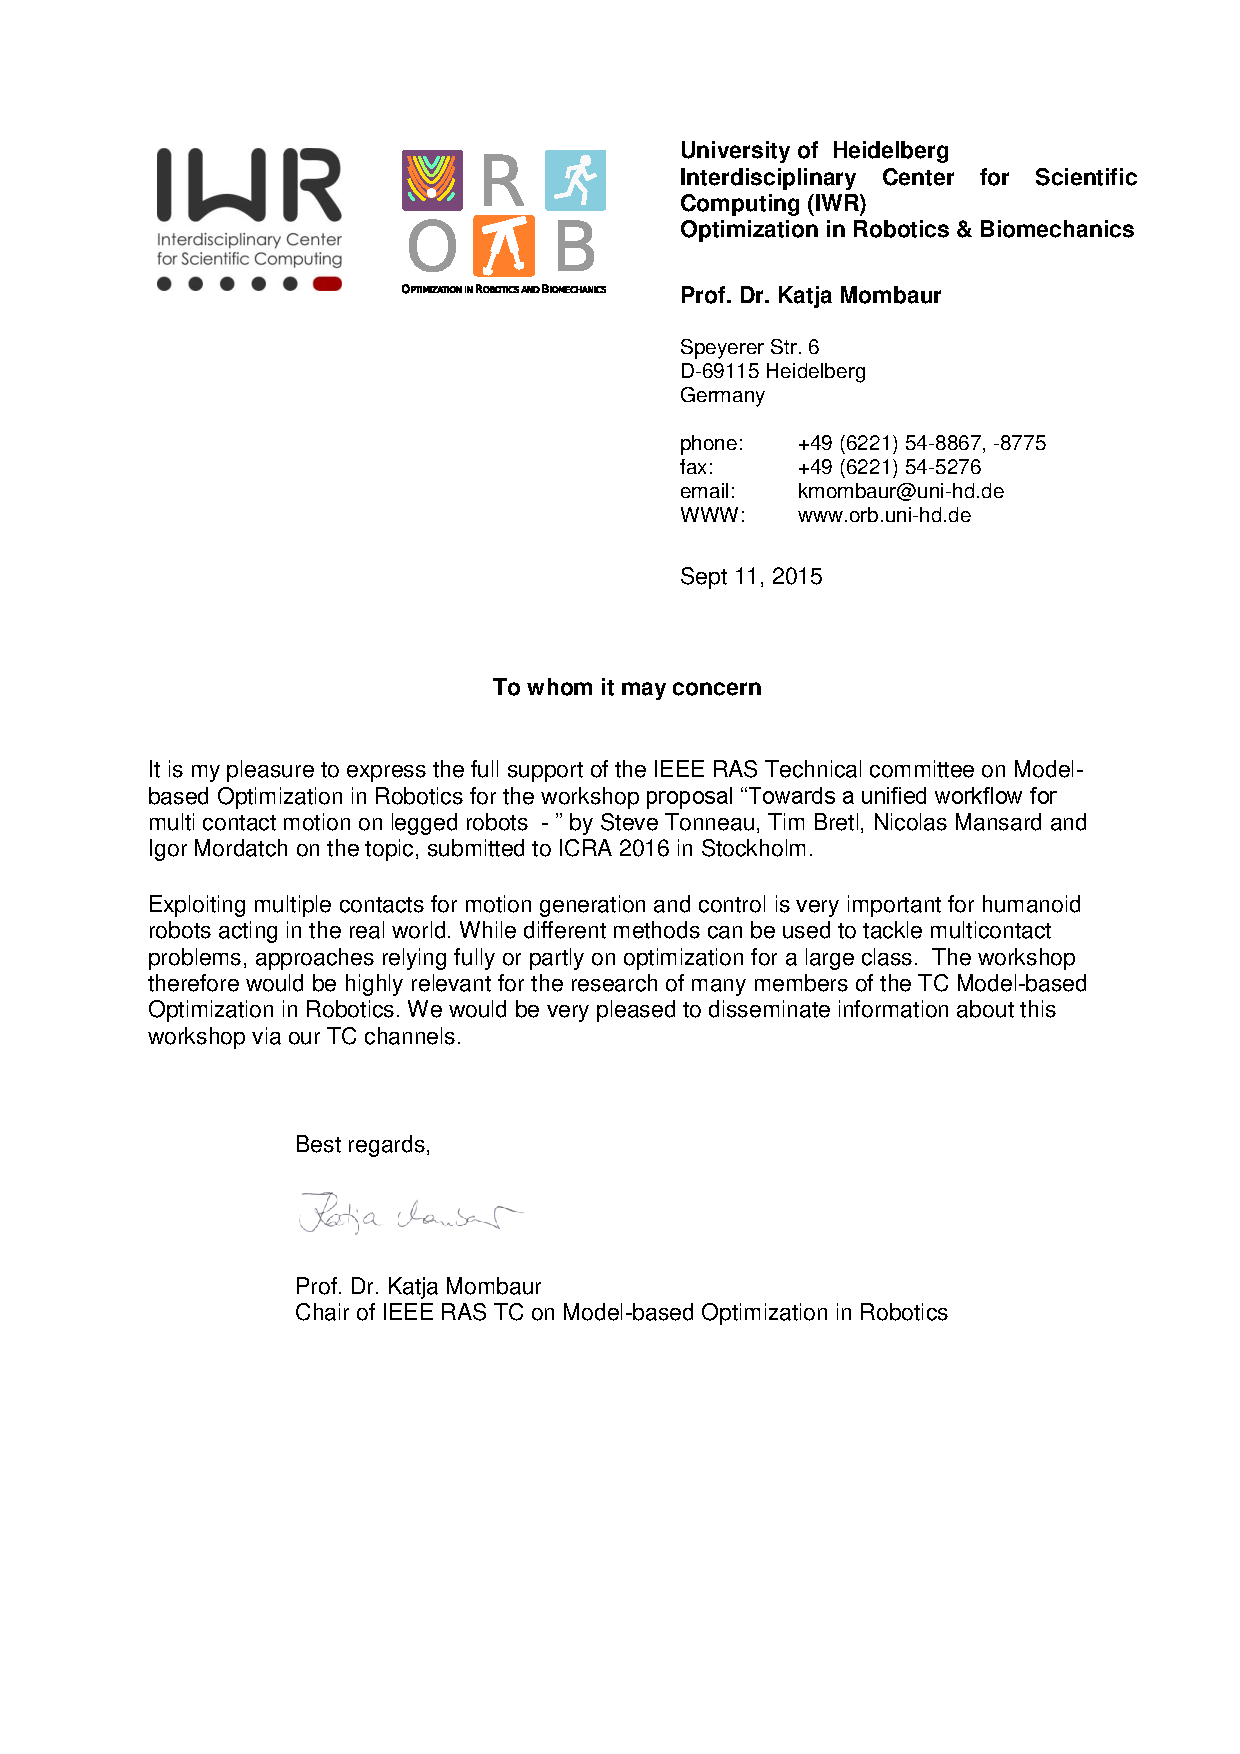
\includepdf[pages=1]{support_icra2016_nicolas.pdf}
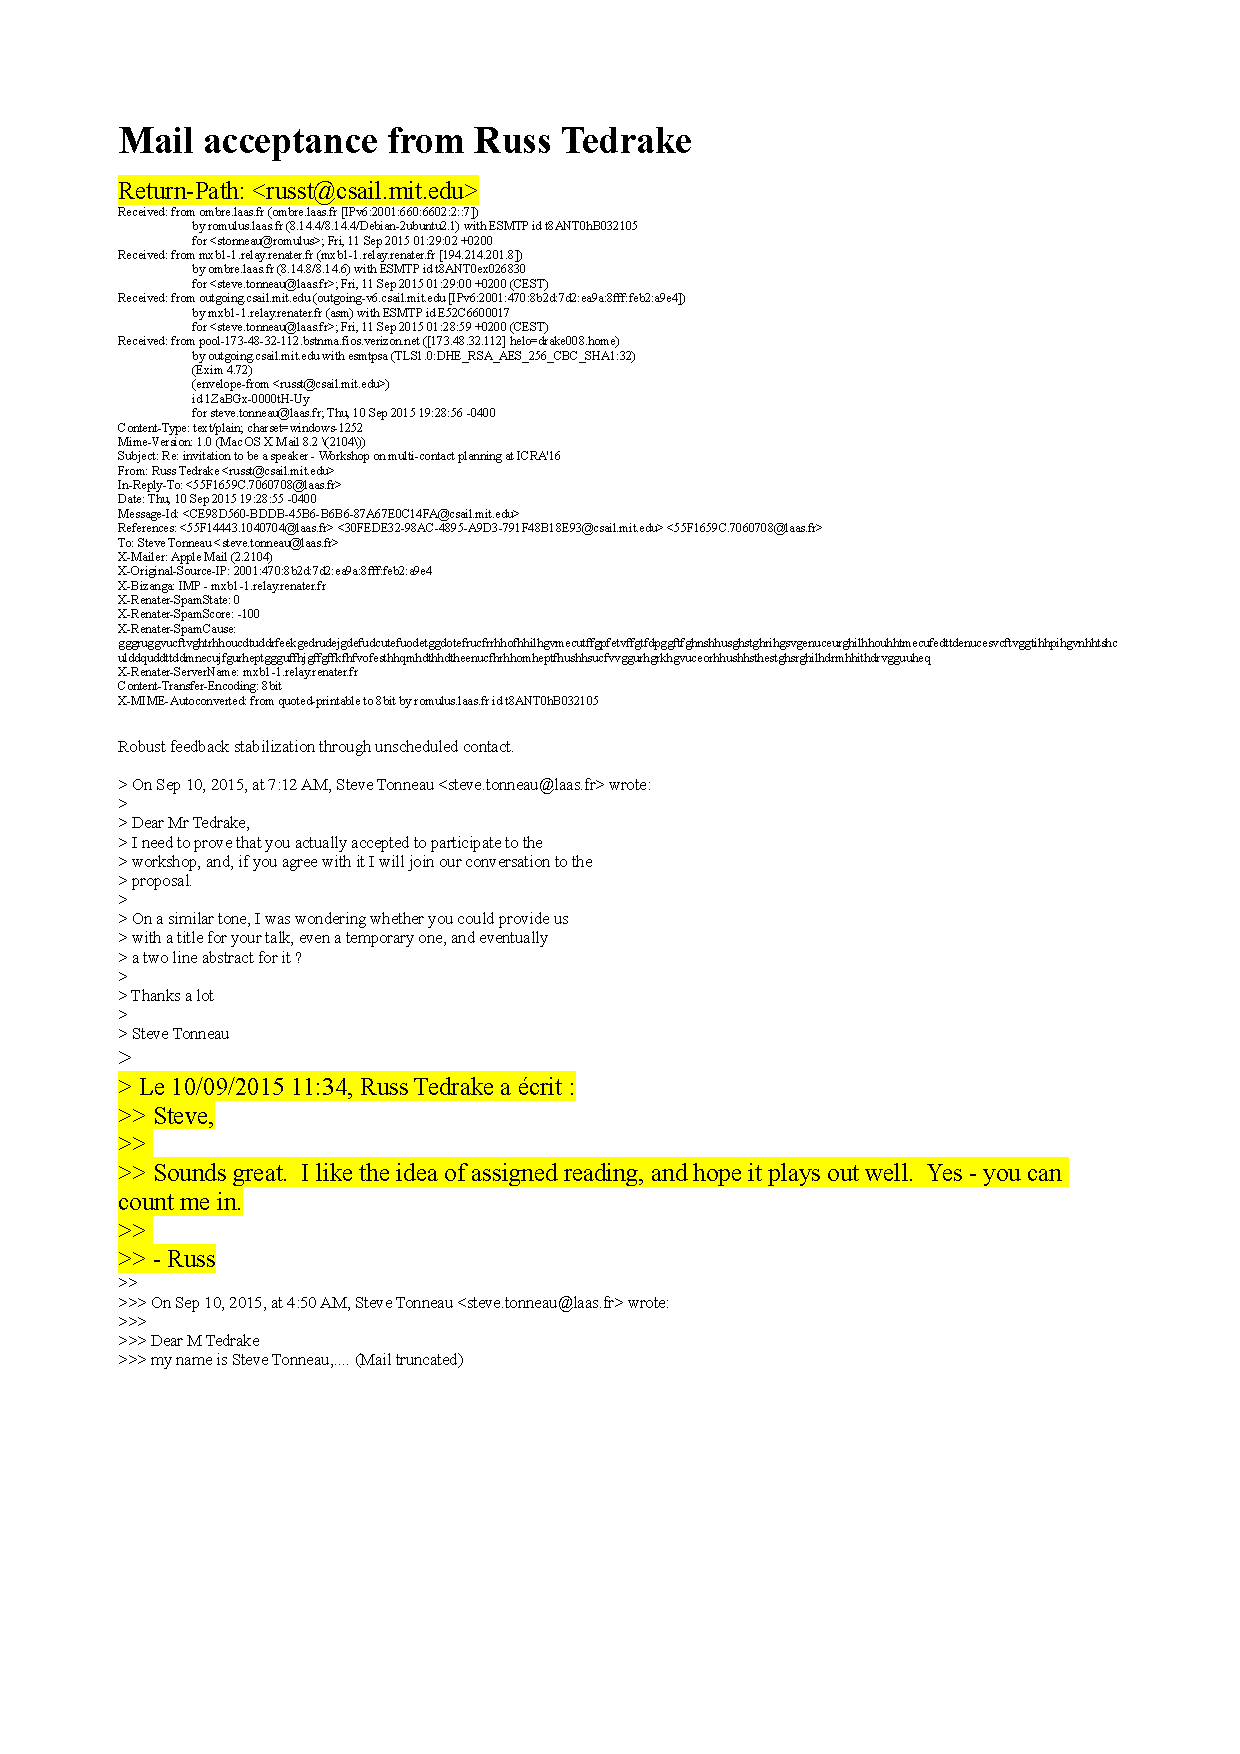
\includepdf[pages=1]{mails.pdf}
\includepdf[pages=2]{mails.pdf}
\includepdf[pages=3]{mails.pdf}
\includepdf[pages=4]{mails.pdf}
\includepdf[pages=5]{mails.pdf}
\includepdf[pages=6]{mails.pdf}


% make the title area
\maketitle




% that's all folks
\end{document}


